\begin{savequote}[8cm]
Alles Gescheite ist schon gedacht worden.\\
Man muss nur versuchen, es noch einmal zu denken.

All intelligent thoughts have already been thought;\\
what is necessary is only to try to think them again.
  \qauthor{--- Johann Wolfgang von Goethe \cite{von_goethe_wilhelm_1829}}
\end{savequote}

\chapter{\label{ch:2-litreview}On the dynamical and thermodynamical mechanisms of the MSD in the Met Office CMIP6 models}

\minitoc


The MSD has relevant implications to farmers in Central America, who are subject to climatic stress due to droughts and are thus affected by the MSD, which is coloquially referred to as 'El Veranillo' in Central America and 'can\' icula' in southern Mexico because the drier period  coincides with the Canis Major constellation appearing in the sky \citep{dilley1996}. In the context of climate change, farmers are already perceiving and having to adapt to changes in the characteristics of the rainy season, such as the timing and strength of the midsummer drought \citep{hellin2017,de2018,harvey2018}. Various communites across country borders have identified and experienced the MSD, which has different names, known as 'El Veranillo' in Central America and because the drier period typically coincides with the Canis Major constellation apearing in the sky, the MSD is also referred to as 'can\' icula' in some regions \citep{dilley1996}.  

This section introduces the main features of the regional climate of Mexico, Central America and the Caribbean. A summary is presented of the literature on the mechanisms that drive the variations of rainfall. The spatial and temporal characteristics of the MSD are also analysed in reanalysis and observations and in HadGEM3 and UKESM1.

\section{Climatological features}
\label{sq:msdclim}
 \begin{figure}[t!]
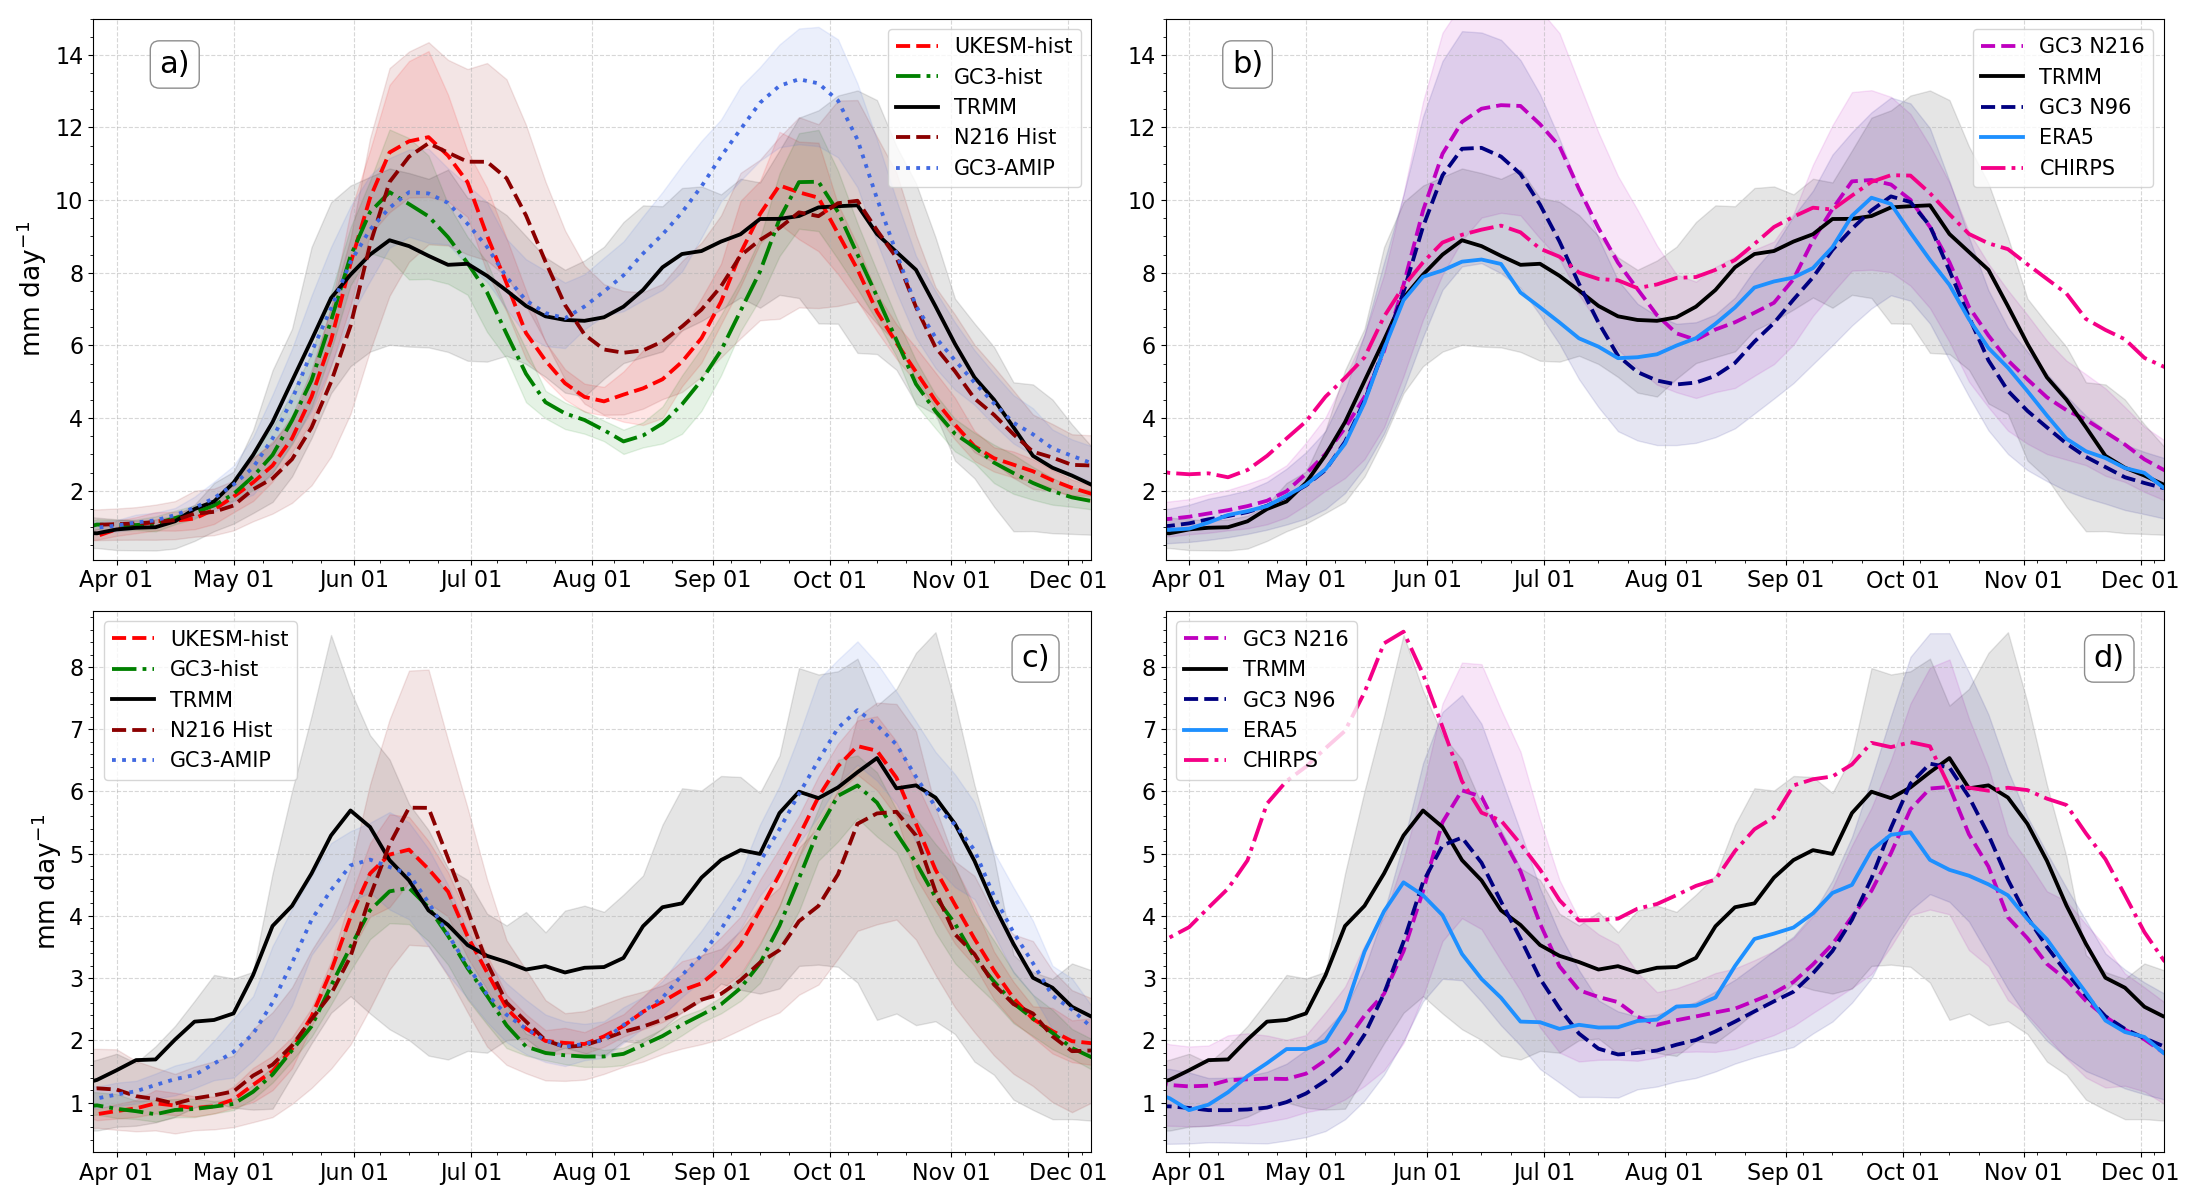
\includegraphics[width=\linewidth]{figures/pmean_f.png}
\caption{Pentad-mean precipitation in (a, b) southern Mexico and northern Central America and (c,d) Cuba. Shading shows uncertainty obtained by bootstrapping or ensemble spread. }
\label{fig:msdcaribb}
\end{figure}

Figure \ref{fig:msdcaribb} shows the pentad-mean seasonal cycle of precipitation in Central America and the Caribbean. The seasonal cycle in both regions follows that of a monsoon, i.e., a dry winter and a wet summer season. In the first region (Figures \ref{fig:msdcaribb}a, b), two precipitation maxima, in June and September, are separated by a decrease in precipitation during July and August, \textit{i.e} the MSD. In Central America, the difference between the first peak (June 15) to the driest pentad of the MSD (Aug 01) is of about 2 mm day$^{-1}$, according to TRMM. 
 The two peak structure in the Caribbean (Figures \ref{fig:msdcaribb}c, d) is characterised by two peaks in May and October with a four-month drier period in between the two peaks  \citep[e.g.][]{giannini2000,gamble2008,angeles2010origins}. In Cuba, the difference between the first peak (June 01) to the driest pentad of the MSD (Aug 01) is of about 3 mm day$^{-1}$ in the TRMM dataset. 
 

 
 \begin{figure}[t!]
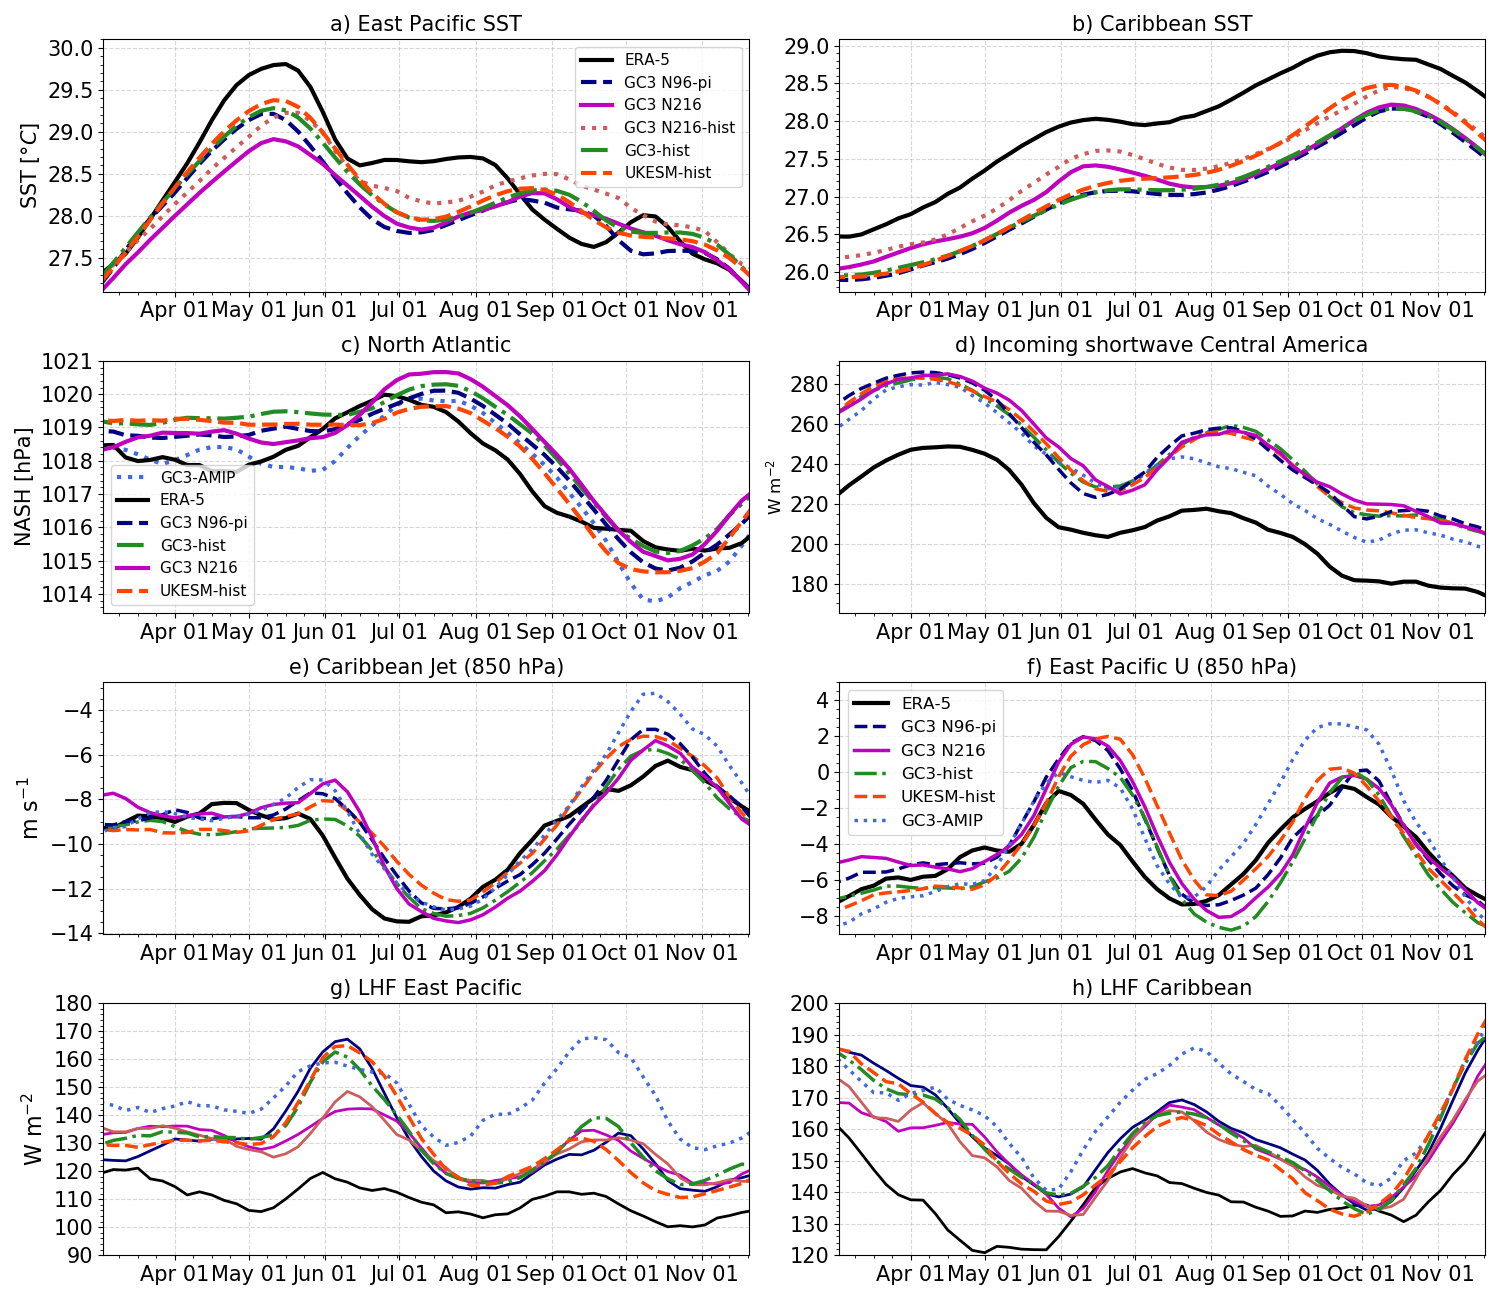
\includegraphics[width=\linewidth]{figures/CSST}
\caption{Pentad-mean seasonal cycle of indices associated with the MSD in Central America and the Caribbean.}
\label{fig:csst}
\end{figure}

Precipitation in these regions depends on several factors such as the seasonal migration of the East Pacific (EP) and Atlantic ITCZs. The SSTs in the Gulf of Mexico, the Caribbean Sea, the western tropical Atlantic and the Eastern Pacific are also very relevant for the seasonal cycle and interannual variations \citep{magana1999,amador2008,straffon2019}. Figures \ref{fig:csst}a, b show the seasonal cycle of SSTs in the EP and the Caribbean Sea. While the EP shows a maximum in SSTs in late May, during the early stages of the monsoon in Central America, the Caribbean SSTs peak in early fall, about five months later. 


%The CLLJ is a strong easterly low-level (925 hPa) that reaches maximum winds speeds of 12 $m\,s^{-1}$ on February and July 
The Caribbean Low-level Jet (CLLJ)is a strong low-level easterly jet in the Caribbean Sea that peaks at the end of June (Figure \ref{fig:csst}e) at the 925 hPa level \citep{amador2008,herrera2015,maldonado2016}. The CLLJ  determines the moisture transport from the Caribbean Sea into the eastern Pacific across the Central American landmass as well as the northward moisture transport into the Gulf of Mexico and Florida \citep{munoz2008,hidalgo2015,maldonado2016}.


%Figure \ref{fig:eof1} shows the climatological summer rainfall in the region and the difference in rainfall between the first peak and MSD and between the second peak and the MSD, characterised by the MSD-MSDO and MSDE-MSD differences. 
%Although the dates of the onset and end of the MSD determined using the WT method are defined using precipitation area-averaged over a relatively small region, the precipitation anomalies associated with the different stages of the seasonal cycle extend to most of Mexico and the Caribbean Sea and Gulf of Mexico. 
%For example, consider the MSDE-MSD differences in the CHIRPS dataset (Figure \ref{fig:eof1}i) where most of northern Central America, southern Mexico, the eastern coast of Mexico shows a positive (+5 mm day$^{-1}$) anomaly. In other words a large region experiences a relatively large increase in rainfall after the midsummer.

\section{Theoretical understanding of the MSD}\label{sq:lit}



Since the first observational descriptions of the MSD \citep[e.g.][]{mosino1966}, studies have aimed to explain the physical mechanisms responsible for causing the observed two-peak seasonal cycle of rainfall. However, 
in spite of extensive research \citep[e.g.][]{magana1999,giannini2000,gamble2008,ryu2014,herrera2015,maldonado2017,straffon2019}, debate remains over which is the leading-order mechanism that causes rainfall to decrease at midsummer and increase again at the end of the summer. Any complete theory or conceptual model must account for the following characteristics of rainfall in these regions. First, the processes that determine the strength of the first peak of rainfall. Second, the timing and strength of the MSD, i.e., what causes rainfall to decrease at midsummer. Finally, the theory must explain the timing and mechanism driving the second increase in precipitation after the midsummer. % why rainfall increases again at the end of the summer, the end of the MSD, and why this happens at this time of the year. 

Studies argue over the roles played by the Atlantic and EP Oceans, and the Caribbean Sea and whether the MSD is caused by two precipitation enhancing mechanisms \citep{karnauskas2013} or a mechanism that inhibits rainfall at midsummer. Furthermore, the close association between the MSD in Central America and in the Caribbean is still disputed \citep{gamble2008}, as most studies suggest that the two regimes are unrelated and therefore two different explanations are required to account for the seasonal cycle of rainfall in these regions. 

\cite{magana1999} and \cite{magana2005} proposed a mechanism driven by radiative-convective feedbacks between the East Pacific SSTs and deep tropical convective clouds. The height and strength of convection, the incoming shortwave and the SSTs are strongly coupled in their framework. %Convection feedbacks with SSTs evaporation and
%moisture flux into the MSD region. 
The peak in  SSTs during May (Figure \ref{fig:csst}a) triggers evaporation and deep convection in the EP ITCZ and Central America (Figure \ref{fig:msdcaribb}).
The high convective clouds produce a radiative cooling effect at the surface due to decreased incoming shortwave radiation (Figure \ref{fig:csst}d).
This cooling  decreases SSTs and deep convective activity and thus accounts for the modest decrease in rainfall during the midsummer.
The second peak in September is then explained by the effect of the less high clouds during July and August, as convective activity decreased, which reduces the cooling effect of the clouds and increases incoming shortwave, SSTs and surface fluxes, and eventually raises precipitation, the so-called second peak \citep{magana1999}.

 However, SSTs in the easternmost Pacific do not increase after, during or at the end of the MSD (Figure \ref{fig:csst}a). 
In fact, the SSTs decrease with the second increase in deep convection and precipitation. The other hypothesis of this theory, referring to the incoming shortwave is also not consistent with observations, as the incoming shortwave only modestly increases during the midsummer (Figure \ref{fig:csst}d). There is perhaps a role for this modest increase in incoming shortwave, but the link to SSTs suggested by this theory does not agree with the reanalysis. 

%have been linked to several sources of seasonal variability,
%but debate is far from uncontroversial as to which is the principal mechanism to account for the MSD.
 Other studies suggest the seasonal evolution of North Atlantic Subtropical High (NASH) and the associated geostrophic flow are the primary cause of the bi-modal regime  \citep[e.g.][]{giannini2000,mapes2005,gamble2008,curtis2008}.The NASH is a subtropical anticyclone in the Atlantic Ocean that shifts southwest early in boreal summer (Figure \ref{fig:csst}c). The expansion and intensification of the NASH in boreal summer, according to this theory, strengthens the low-level trade winds, controlling the seasonal cycle of the CLLJ, therefore cooling the SSTs, through the effect of wind stress and mixed-layer mixing.
The SST cooling diminishes evaporation and therefore low-level moisture which leads to less precipitation.


 \cite{herrera2015} shows that during the drier months in Central America, stronger convective activity is found west of the Central American coast.  This evidence suggests that the coupling of EP SSTs to the gap flow that originated from the CLLJ in the Caribbean Sea controls the location of ascending and descending motions, thereby explaining some features of the Central American MSD. 
\cite{herrera2015} argues also that the exit region of the CLLJ is located to the east of the region of strongest MSD signal, which suggests that the moisture divergence effect over the central American MSD is minimal. 


A different mechanism, proposed by \cite{karnauskas2013}, argues that the biannual crossing of the solar declination angle can control precipitation to the extent of explaining the bimodal characteristics of the seasonal cycle. In this mechanism, the MSD is driven by two precipitation enhancing periods that are separated by a relatively normal, and drier, period. This theory differs from those previously discussed which explained the MSD through mechanisms that inhibit convective activity in the midsummer whereas \cite{karnauskas2013} argues that the solar declination angle that crosses twice through Central America, once during June and a second time during September, increases convective activity during each crossing. The variations of incoming shortwave radiation associated with the declination angle modulate the SSTs, surface fluxes and therefore convective activity. In other words, the first crossing poses a strong increase to incoming shortwave that increases the SSTs, evaporation and precipitation, i.e., the first peak. The second crossing, similarly, explains the second peak as the second increase in incoming shortwave promotes more deep convection than during the MSD. However, as shown in Figure \ref{fig:csst}a and as discussed for the radiative-convective feedback of \cite{magana1999}, SSTs do not increase in the East Pacific in the late summer and the second increase in incoming shortwave is only modest in the reanalysis (Figure \ref{fig:csst}d). 


Other mechanisms have been proposed arguing that the MSD is a result of the double crossing of the Intertropical Convergence Zone (ITCZ), the result of vertical wind shear affecting convective instability or the Saharan dust controlling  the microphysics of clouds \citep{angeles2010origins}.
For instance, \cite{perdigon2019} also finds a link betwen the frequency and spatial distribution of the first peak rainfall rates and the Madden-Julian Oscillation. 

  \begin{figure}[t!]
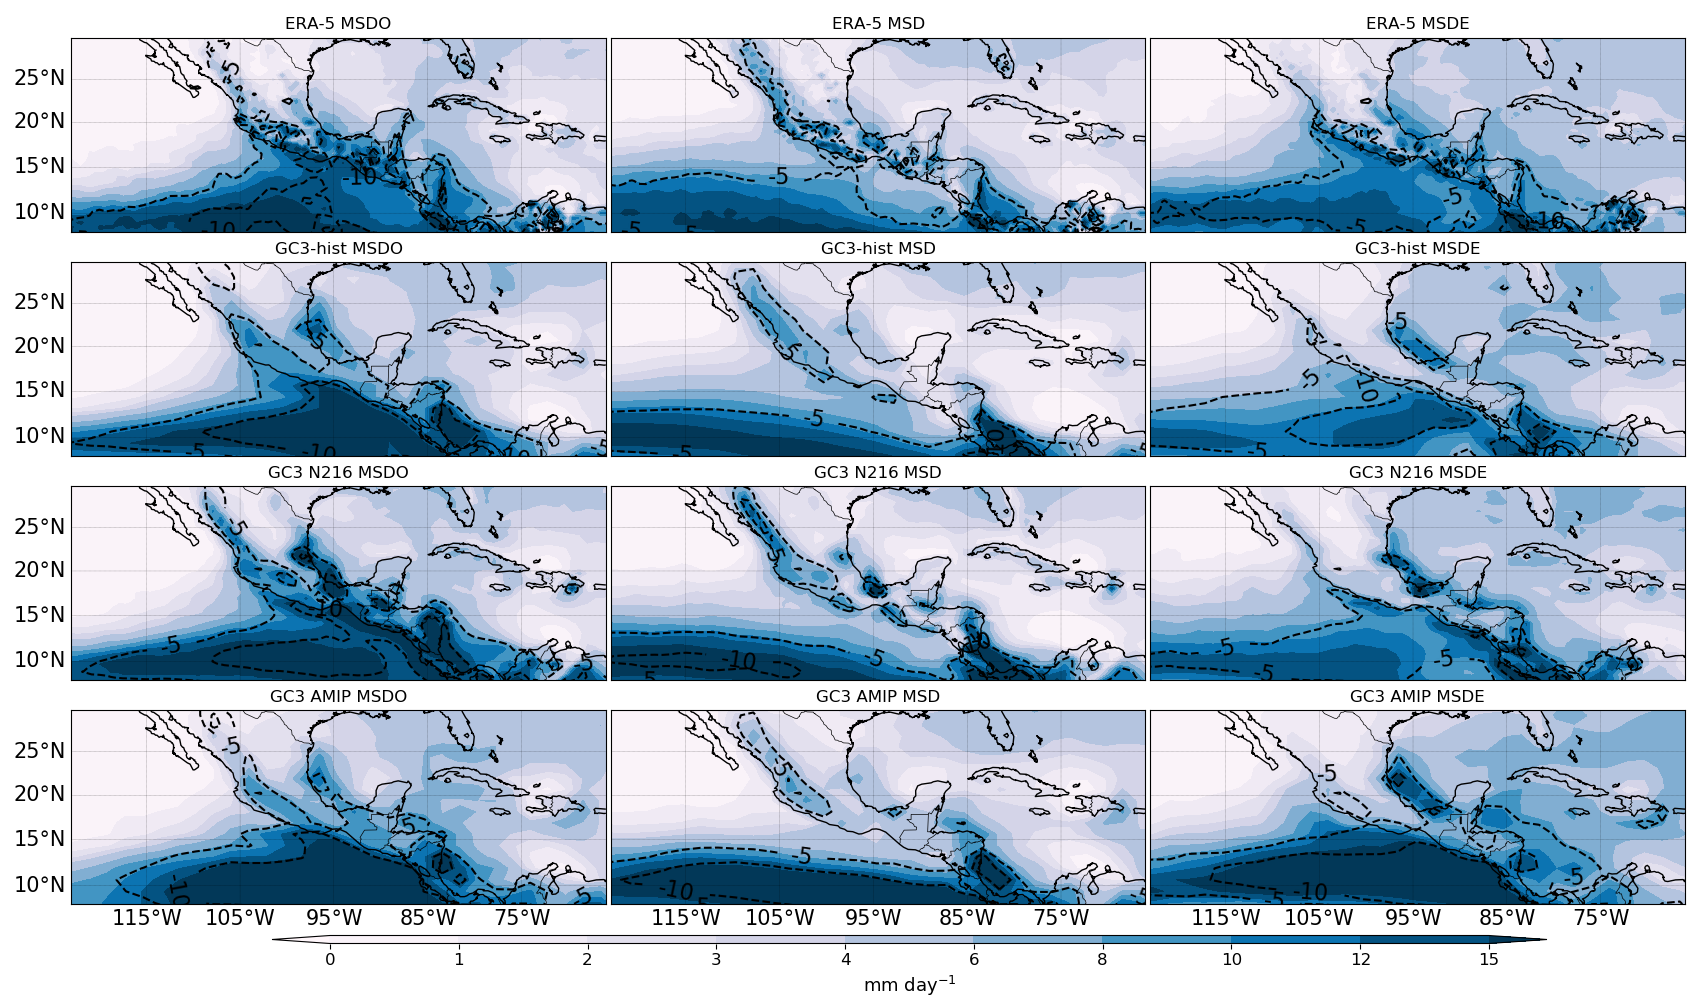
\includegraphics[width=\linewidth]{figures/modcompar_dif2pr3.png}
\caption{Intra-seasonal march (left to right) of precipitation (shaded) and vertical velocity ($\omega$) at 500-hPa in ERA-5, GC3-hist, GC3 N216 and GC3 AMIP (top to bottom). For each dataset, the periods shown are 10 days prior to the onset of the midsummer drought (MSDO), the MSD period and the 10 days after the end of the MSD (MSDE).}
\label{fig:eof2}
\end{figure}


\subsection{ On the mechanisms of the MSD in the UK Met Office models}
\label{sq:chap3}

Biases in the strength and position of the EP ITCZ in Global Coupled Models (GCMs) \citep{bellucci2010,li2014,schneider2014} are a major reason for biases in the model representation of rainfall in Central America  \citep{rauscher2008}. 

\cite{ryu2014} analyzed the performance of CMIP3 and CMIP5 models and found that the majority of CMIP5 models were unable to represent the total annual rainfall and the seasonal cycle of the MSD. \cite{ryu2014} also finds that models that simulate a bimodal distribution of rainfall, HadGEM2-A for example, also show an accurate seasonal cycle of the NASH and the CLLJ. However, an exhaustive analysis as to whether these features are actually driving mechanisms for the MSD in GCMs as in observations is missing from the literature. 


The CMIP6 Met Office models, HadGEM3 and UKESM1, are amongst the first models to simulate a bimodal regime in both Central America and Cuba (Figure \ref{fig:8}a and \ref{fig:msdcaribb}). 
In Central America and southern Mexico, the models simulate a wetter-than-observed first peak of precipitation and a drier MSD period.
% 
The so-called second peak of precipitation found in late August is simulated in close agreement with TRMM, except in the AMIP experiment which has a far too strong second peak mean precipitation rate.
% The seasonal cycle and other characteristics of the MSD showed noticeable differences between the different experiments analysed in this study. 


%\subsubsection{Climatological features of the MSD in UKESM1 and HadGEM3}
%Rainfall during the first peak has been too wet in these models since CMIP3, suggesting a persistent wet bias in this region associated with the East Pacific ITCZ \citep{ryu2014,mulcahy2018}. 
Figure \ref{fig:eof2} shows the distribution of rainfall in the different stages of boreal summer in different CMIP6 experiments and ERA-5. 
The main feature, the East Pacific ITCZ shows the maximum rainfall rates (>15 mm day$^{-1}$ in the models) and strong mid-level ascent (-0.1 Pa s$^{-1}$). Prior to the MSD, rainfall extends from the easternmost Pacific ITCZ into the North American continent. Therefore, the positive bias during the first peak over land is associated with the biased wetter EP ITCZ.  However, during the MSD, rainfall decreases over land remaining only above 10 mm day$^{-1}$ south west of the coastline in the models.



%For example, the Atlantic ITCZ biases have been shown to be directly affected by processes in the convective scheme \citep{bellucci2010}, such as the treatment of entraintment and moisture-cloud feedbacks \citep{oueslati2013,li2014}. 

The wetter EP ITCZ is a common feature of GCMs, including the Met Office models, which results from multiple biases in the radiative and convective schemes \citep{oueslati2013,li2014}. %For instance, the oversensitivity of convection to SSTs in models is a known problem with tropical climate modelling \citep{}.
% The entraintment parameter and cloud-radiative feedbacks have also been shown to play a role in these biases . 
 In UKESM1 and HadGEM3 several biases exist in the radiative balance in the easternmost Pacific Ocean. A positive bias in incoming shortwave in Central America of about 15\% and a cold SST bias in both East Pacific and Caribbean Sea SSTs are observed in Figure \ref{fig:csst}. Increased incoming shortwave but cooler SSTs require increased surface fluxes to maintain energy balance. These higher latent heat fluxes (LHFs) in the models in both basins (Figs. \ref{fig:csst}g, h) are almost 40\% larger than in ERA5 during the first peak of rainfall. The models also exhibit a larger seasonal cycle of the fluxes than the reanalysis. GC3 AMIP is the only simulation to also show a significantly positive bias in LHFs during the second peak of rainfall in the EP but also at the end of MSD in the Caribbean Sea. 


In all the model experiments, the ITCZ prior to the MSD period is stronger than in ERA5 by more than 5 mm day$^{-1}$, whereas after the MSD rainfall in the coupled models on the western coast of Central America agrees well the ERA5. 
This analysis suggests that the biases shown in Figure \ref{fig:7} are mostly coming from the period prior to the MSD. The models reasonably simulate the decrease in rainfall during the MSD (Figure \ref{fig:eof2}) followed by the second increase or peak. 
Note that GC3 AMIP, forced by very similar SSTs as ERA-5, simulated a much larger mean precipitation in the ITCZ during MSDE in contrast to the coupled models. This large positive bias in simulated rainfall in the East Pacific in GC3 AMIP corresponds to the larger than observed second peak observed in Figure \ref{fig:msdcaribb}a. 


 \begin{figure}[t!]
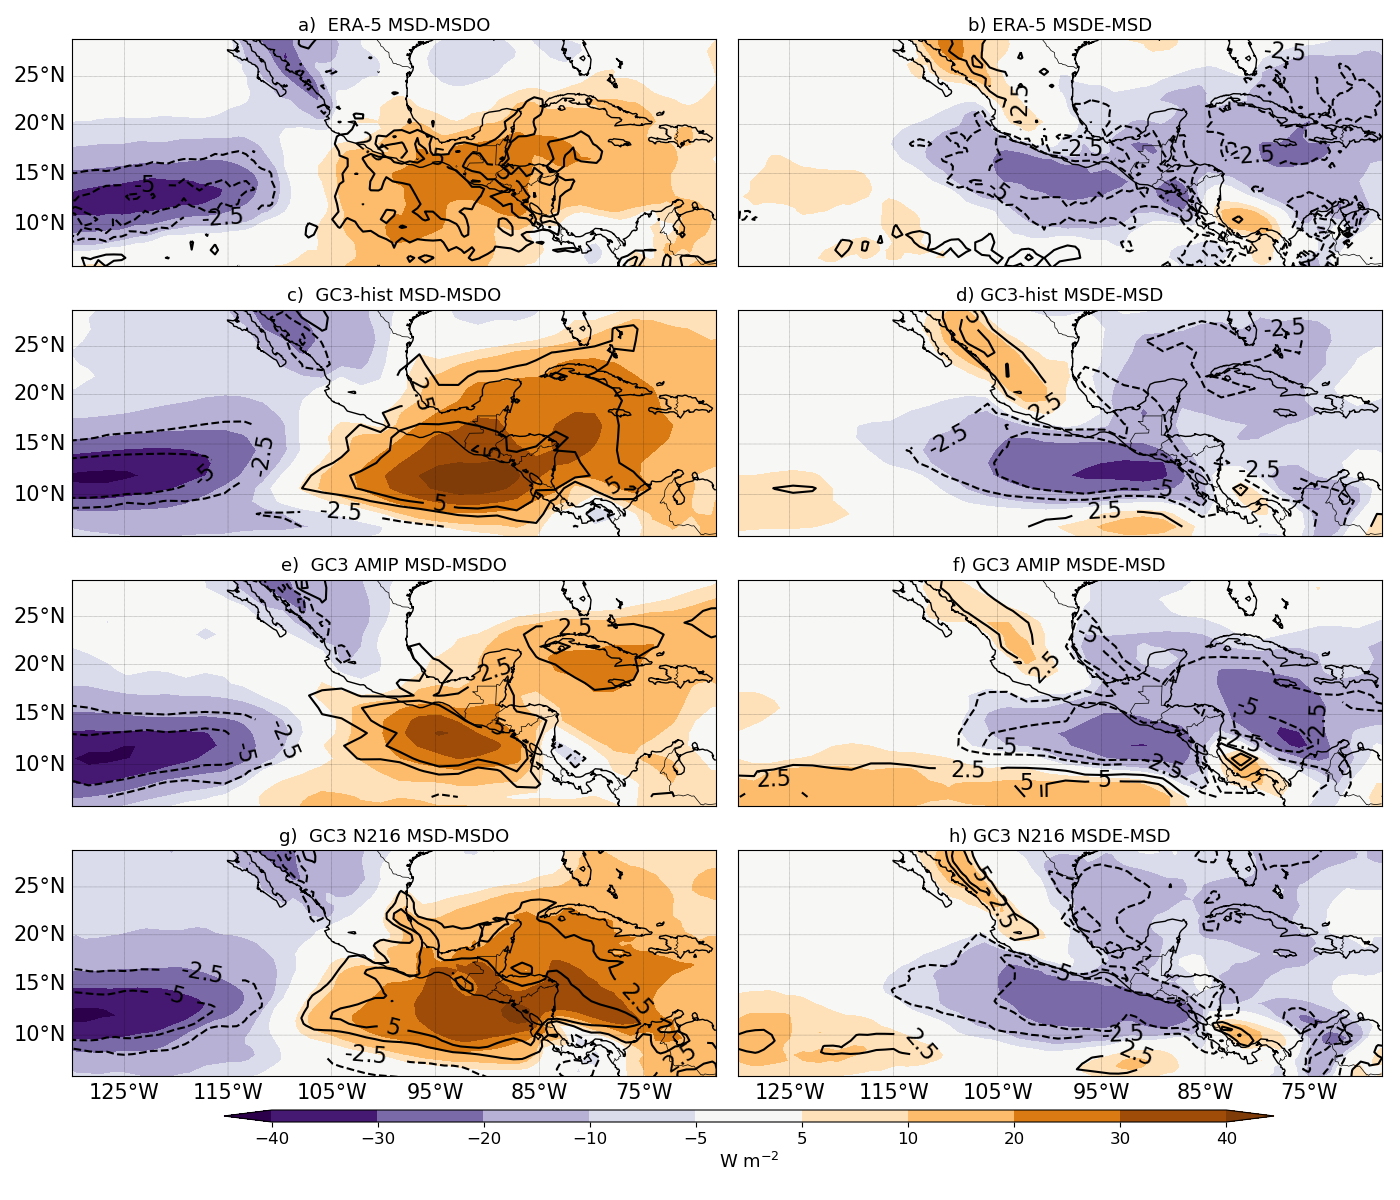
\includegraphics[width=\linewidth]{figures/fig4_olrdiff.png}
\caption{Out-going longwave radiation (OLR) [W m$^{-2}$] (shaded) and $\omega$ 500-hPa [$10^{-2}$ Pa s$^{-1}$] (line contours) differences between the MSD and MSDO and the MSDE and MSD.}
\label{fig:msdolranom}
\end{figure}


 \begin{figure}[t!]
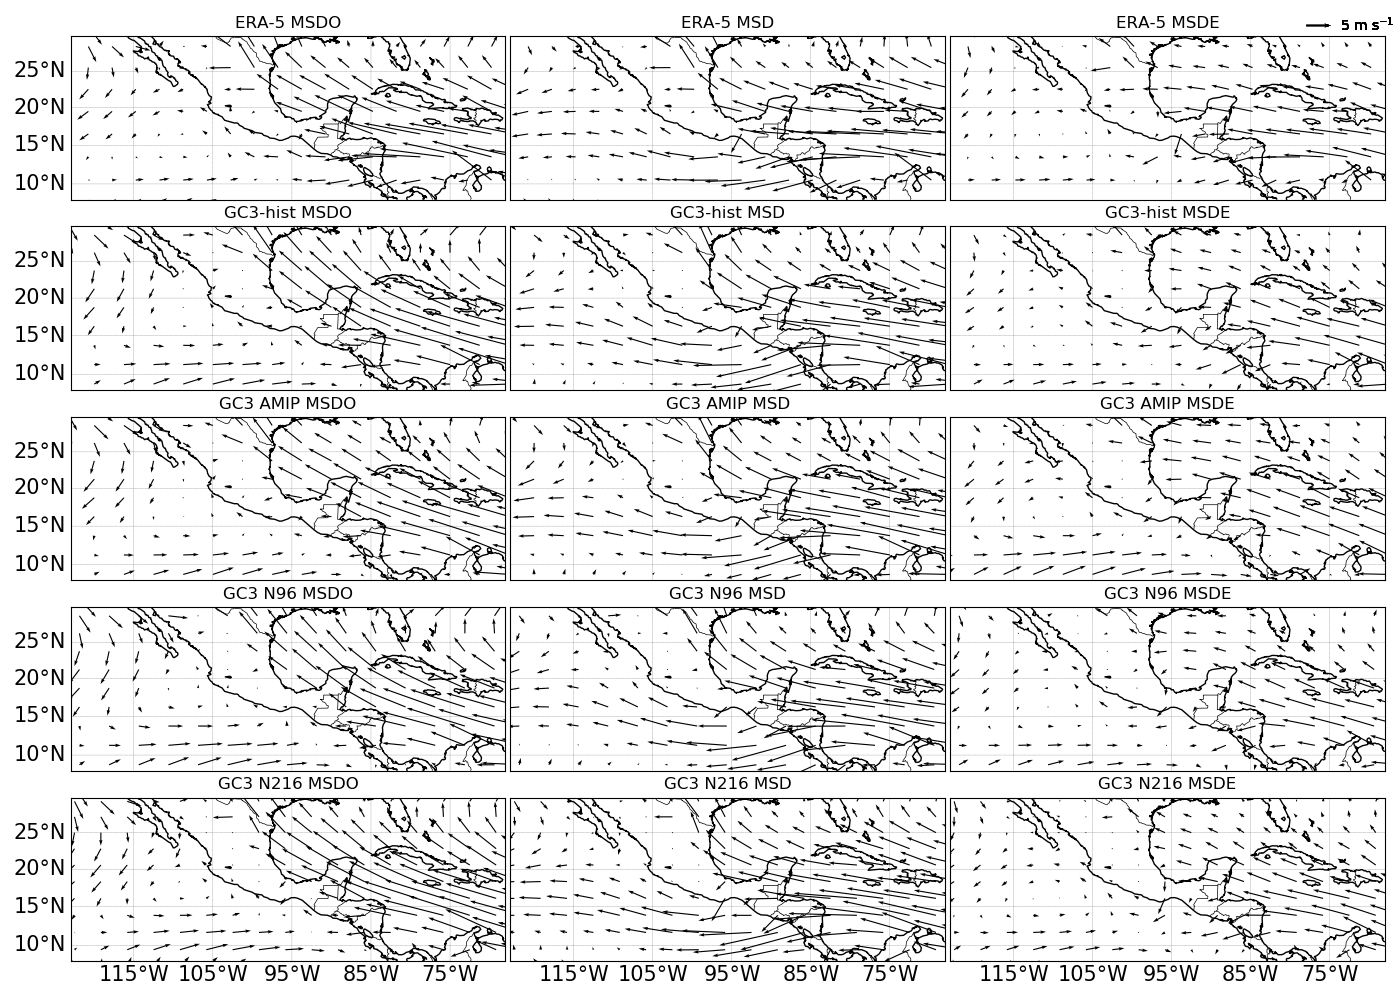
\includegraphics[width=\linewidth]{figures/modcompar_dif2u3}
\caption{As in Figure \ref{fig:msdolranom} but showing wind vectors at the 850 hPa level. }
\label{fig:msduanom}
\end{figure}


Composites prior to the onset of the MSD, during the MSD and after the MSDE were computed for several diagnostic variables. The periods were separated using the WT method to determine the dates of the MSDO and MSDE in ERA5 and the climate model output.
Figure \ref{fig:msdolranom} shows the composite differences between the period of the MSD and of the two peaks in out-going longwave radiation (OLR) and vertical velocity ($\omega-500$) at 500 hPa.
The positive OLR and $\omega$ anomalies in the MSD-MSDO panels in southern Mexico and northern Central America are indicative of decreased height of convection and decreased ascent, in agreement with the MSD being the drier period. These positive anomalies in the continent are accompanied by negative OLR and $\omega-500$ anomalies west of the continent, around 125$^\circ$W. 
%These anomalies are stronger in the simulations (e.g., Figure \ref{fig:msdolranom}c). 


The MSDE-MSD panels show the difference between the second peak of rainfall and the drier MSD period. Negative OLR and $\omega$ anomalies indicate stronger and higher convection over a wide region including the easternmost Pacific Ocean, southern Mexico, northern Central America Cuba and the Caribbean Sea.  
Note also the region of the North American Monsoon, on the northwest corner of Mexico and the southernmost US, as the MSD-MSDO difference suggests increased convective activity in the North American Monsoon region and 
MSDE-MSD the opposite. 

 \begin{figure}[t!]
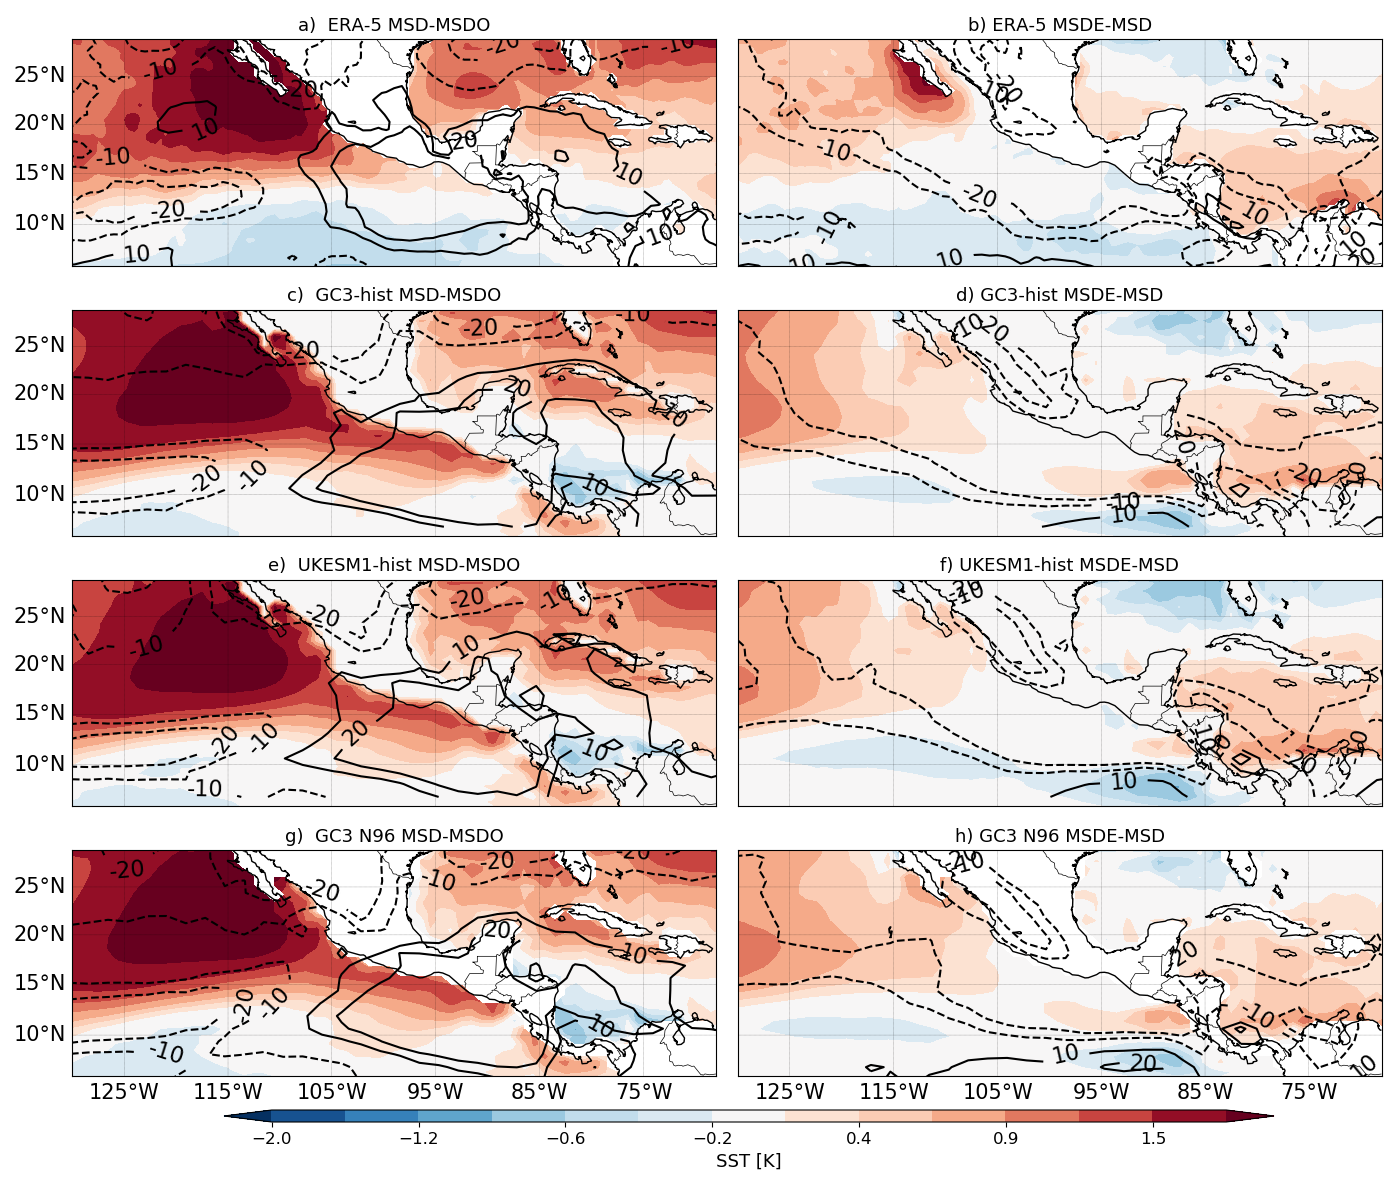
\includegraphics[width=\linewidth]{figures/fig4_sstdiff}
\caption{As in Figure \ref{fig:msdolranom} but the anomalies are shown for SSTs [K] (contours) and incoming shortwave radiation [W m${-2}$] at the surface (line-contours). Incoming shortwave is defined such as negative differences imply less incoming shortave and positive anomalies represent more incoming shortwave at the surface. }
\label{fig:msdsstanom}
\end{figure}

Similarly, Figure \ref{fig:msduanom} shows the low-level wind field during the three stages of the MSD. In ERA-5, prior to the MSD the wind flow in the Caribbean shows strong easterlies that flow into the Gulf of Mexico and southeastern US but very weak winds in the EP (see Figure \ref{fig:csst}f). During the MSD, the winds in the EP become modestly strong eaterlies associated the easterly flow from the Caribbean Sea that crosses over Costa Rica and Nicaragua from the Caribbean Sea to the East Pacific. Note that the easterlies converge towards the region at 125$^\circ$W where OLR and $\omega$ anomalies suggest increased ascent. 

By the end of the MSD the easterlies in ERA5 weaken substantially on the western coast of Central America and in the Caribbean Sea.
The simulations seem to generally reproduce the characteristics of the wind field with some differences worth mentioning. For instance, prior to the onset of the MSD, all the simulations show a modest westerly wind flow in the east Pacific at 10$^\circ$N, which can also be seen in Figure \ref{fig:csst}f, which is not observed in ERA5.
After the MSD ends, most simulations show a very weak westerly flow in the East Pacific, close to ERA5; however, GC3 AMIP shows a modest westerly wind converging towards the west coast of Nicaragua. This low-level convergence may be forcing the increased convective activity and precipitation during this time in GC3 AMIP.

The SSTs and incoming shortwave radiation are key elements for explain the seasonal cycle of the MSD, according to previous theories summarised in section \ref{sq:lit}. 
Figure \ref{fig:msdsstanom} shows the corresponding SST and incoming shortwave anomalies during the different stages of the seasonal cycle. % MSD-MSDO and MSDE-MSD anomalies. 
From the first peak to the MSD, a positive SST difference of +1.5 K in the Gulf of California and the western coast of the Baja California Peninsula is observed in reanalysis and the models. The differences appear as a sharp SST meridional gradient pattern around 115$^\circ$W. 
During this stage, the incoming shortwave increases in Central America, which agrees with Figure \ref{fig:csst}d. 
Note the negative incoming shortwave differences west of Central America at 125$^\circ$W, the region of negative OLR and $\omega$-500 hPa anomalies where low-level winds converge, all of which supports the notion of increased convective activity that reduces incoming shortwave west of the continent. This feature was noted by \cite{herrera2015}. 

 \begin{figure}[t!]
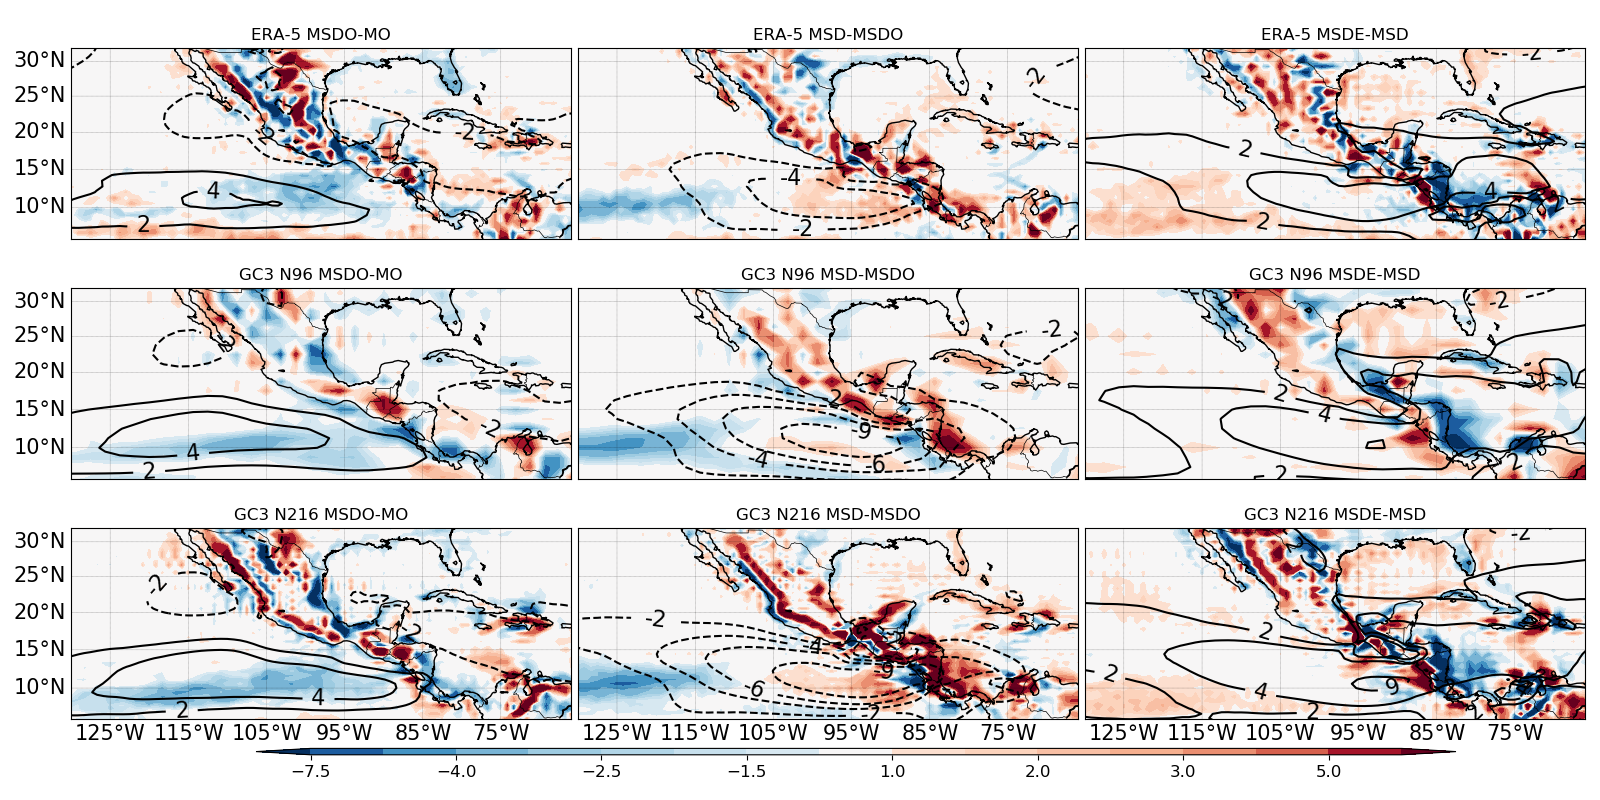
\includegraphics[width=\linewidth]{figures/modcompar_dif2mfc3}
\caption{As in Figure \ref{fig:msdolranom} but showing in shading, moisture flux divergence $\nabla \cdot \vec{u}q$ at the 850 hPa level with units of $10^{-7}$ s$^{-1}$ kg / kg and zonal wind anomalies (line contours) in m s$^{-1}$.  }
\label{fig:msdmfcanom}
\end{figure}

After the MSD, the western coast of the Baja California Peninsula continues to warm and the East Pacific continues to cool, in contrast to previous suggestions \citep{magana1999,magana2005,herrera2015}. Meanwhile, the Caribbean Sea warms by 1 K and the northern Gulf of Mexico slightly cools down. The incoming shortwave differences show a regional-scale decrease in incoming shortwave, as the summer draws to an end. 
These SST differences indicate that the meridional SST gradient in both the EP and Caribbean Sea and Gulf of Mexico is greatly modified during the stages of the MSD. 


The main dynamical argument put forth to explain the MSD is centred around variations in the moisture flux convergence (MFC), argued to be driven by the Caribbean-Low Level Jet \citep[see e.g.][]{gamble2008,herrera2015,martinez2019}. The MFC and zonal wind variations in each stage of the MSD is shown in Figure \ref{fig:msdmfcanom} for ERA-5 and two simulations. The low-level MFC increases from monsoon onset (MO) to the first peak period (MSDO) in the EP. This anomaly in MFC corresponds to a region of positive zonal wind anomalies indicative of weaker easterly flow.
 This zonal wind anomaly from MSD to MSDO is much stronger in the models.  
The MSD-MSDO difference shows a strong positive MFC anomaly across southern Mexico and most of Central America. 

In turn, the MFC anomalies associated with the end of the drier period, observed as the MSDE-MSD anomalies,  show negative values, suggesting increased moisture flux, over southern Mexico and northern Central America.
Increased moisture flux during the transition from the MSD to the second peak agrees well with the precipitation differences during these periods.  The MSDE-MSD zonal wind anomalies in the EP show positive zonal wind anomalies, suggesting a weakened easterly wind flow (see also Fig. \ref{fig:msduanom}). 

The MSD in Central America and southern Mexico has been strongly linked to the strengthening of the CLLJ \citep{herrera2015}. The maximum zonal wind observed in the CLLJ is found at the very end of July (Fig. \ref{fig:csst}e), synchronized with the start of the MSD. 
The zonal wind anomalies in the MSD-MSDO panels in Figure \ref{fig:msdmfcanom} show that easterlies in the Caribbean Sea do not strengthen by more than 2 m s$^{-1}$ from the first peak to the MSD. Only in the models is there a modest negative anomaly at the westernmost Caribbean Sea. In other words, while the peak of the climatological CLLJ coincides with the climatological timing of the onset of the MSD, these composite analyses constructed by more specifically separating the MSD periods does not show relevant variations in the zonal wind of the Caribbean Sea. 
The drier MSD period does coincide with stronger easterly flow over the eastern Pacific, which may be associated with the weaker MFC over land. %The end of the MSD then coincides when the easterly winds weaken. 

\subsection{Summary and discussion}\label{sq:sumdiscuss}


 \begin{figure}[t!]
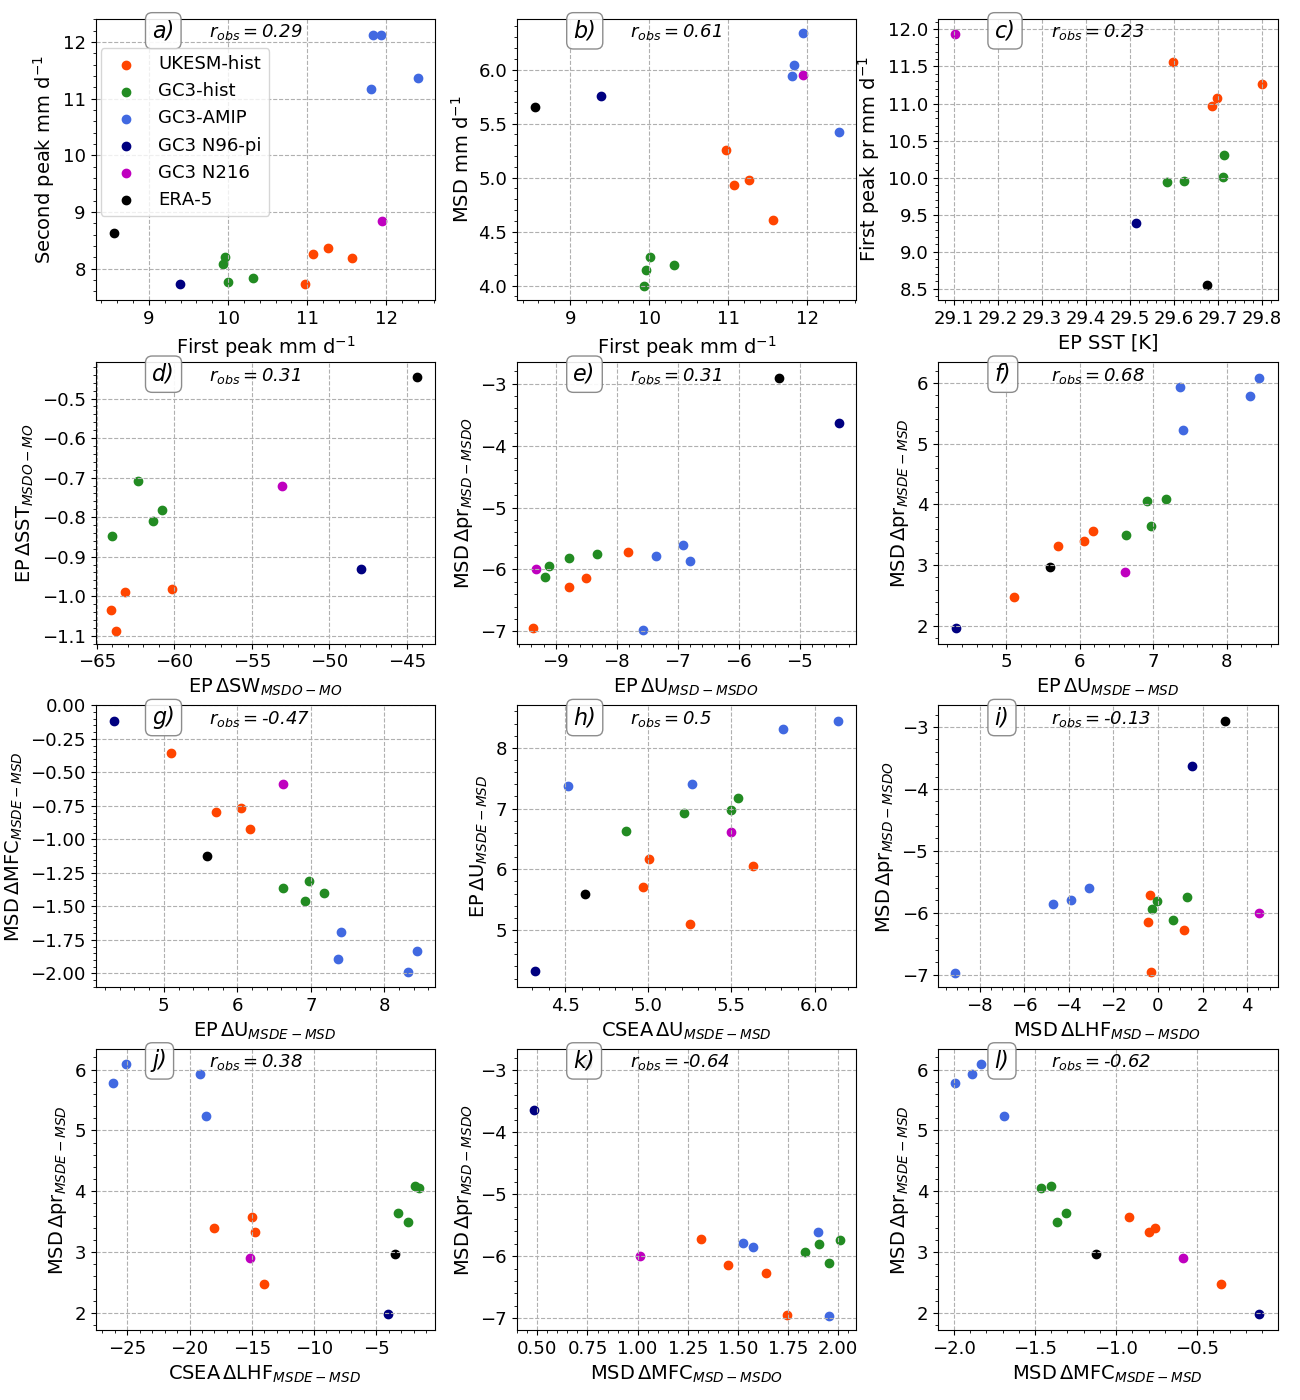
\includegraphics[width=\linewidth]{figures/scatter}
\caption{Scatter plot of the (a, b) area-averaged precipitation over land  (Box in Figure \ref{fig:7}) during the different stages of the MSD. (c) scatter of the East Pacific SSTs against  the precipitation over landduring the first peak period. (d-l) show the scatter differences in several variables between the different stages of onset of the MSD (MSDO), the drier MSD and the end of the MSDE. The differences are shown for area-averaged quantities in the East Pacific (EP), the Caribbean Sea (CSEA) and overland (MSD) as above. The units for $\Delta$U are [m s$^{-1}$], $\Delta$MFC [10$^{-11}$ s$^{-1}$], $\Delta$SW and $\Delta$LHF [W m$^{-2}$] and $\Delta$pr mm d$^{-1}$.   The Pearson correlation coefficient for the 38 yr of  reanalysis or observations ($r_{obs}$) is shown for each panel. }
\label{fig:scatter}
\end{figure}

The midsummer drought  is a  prominent feature of the seasonal cycle of rainfall of southern Mexico, northern Central America and the Caribbean. The average 20\%  decrease during the midsummer compared to the wetter periods of early and late summer is a rare feature of monsoon regions that has important implications for agriculture and water management  \citep{hellin2017,de2018,harvey2018}. 

Climate predictions of the MSD, particularly those concerning whether this "drought" will become more pronounced in the following years, are not trustworthy because of several reasons. 
One factor is the current limitation in the understanding of the physical processes that cause the MSD (section \ref{sq:lit}) as debate still exists over which large or regional-scale processes are most important to explain the increases and decreases of precipitation over intraseasonal time-scales.
Secondly, methods used to diagnose the timing and strength of the MSD typically deal with monthly-scale metrics, which would obscure subtle trends and processes that have an effect on shorter time-scales. 
Also relevant is the fact that climate models used to produce the predictions show significant biases in the EP ITCZ and the seasonal cycle of rainfall in the region, in fact, most CMIP3 and CMIP5 models did not show a bimodal signature in the seasonal cycle. Models that do not have a climatological MSD cannot provide a prediction for this regime in future climate. 

For these reasons, this section analysed the CMIP6 simulations from the Met Office models, UKESM1 and HadGEM3, aiming to understand the causes of the biases in the seasonal cycle. Furthermore, these models are better compared to CMIP3 and CMIP5 cohorts since UKESM1 and HadGEM3 actually simulate a bimodal precipitation regime in these regions. 
The purpose of this investigation is to use these climate models to better diagnose the relevant biases for the representation of the MSD but also understand the processes that these models are capturing leading to the MSD, in order to, hopefully, also highlight the dynamics of the MSD in general. 
%Therefore,this section and future thesis chapter evaluates the similarities and differences between reanalysis and model experiments. 
% For varios reasons, determining the timing and strength of the MSD is very important to agricultural practices,  and water management planning. 





%The different experiments showed notable differences in the precipitation amount in the MSD seasonal cycle.  The first peak, however, appears to be modestly related  to the precipitation amount during the MSD in the models and in observations ($r=0.6$) suggesting that the wetter the first peak the wetter the MSD period.  


 The wavelet transform method was developed to determine the pentads of onset and end of the MSD.  For instance, Figures \ref{fig:scatter}a,b show the scatter of the mean precipitation during the first peak against second peak and first peak against MSD in all the simulations and ERA5. The magnitude of the first and second peaks appear to be unrelated in these models and in observations, which would suggest that the processes driving each peak are not exactly the same.
 Similarly, composite analysis of various diagnostics during the different stages of the seasonal cycle was done, for instance,  OLR composites showed that the MSD is not a local feature in a small region of southern Mexico but extends throughout a wide range of North America,  from central Mexico through Belize, Guatemala, El Salvador, Honduras, Nicaragua, and northern Costa Rica. % Although the MSD has been documented in all these regions \citep{magana1999,perdigon2018}, these composites showed a synchronicity in the precipitation anomalies and a larger extent to the western Mexican coastline that were not previously shown, to our knowledge. OLR anomalies between the second peak and the MSD also showed a simultaneous increased convective activity in the Caribbean. 
 
 This composite approach also allowed to test previously proposed hypotheses by analysing the differences between model experiments and the observed variability in the characteristics of the precipitation at each stage of the MSD.
 For example, \cite{magana1999} proposed a mechanism that explains the MSD through SST-cloud feedbacks. In this hypothesis, shortwave, SSTs and precipitation are strongly coupled in the EP Ocean. The first peak of precipitation in southern Mexico and Central America would then be associated with the EP SSTs prior to the onset of rainfall. 
 Figure \ref{fig:scatter}c shows that EP SSTs prior to onset do not explain the inter-model differences in the magnitude of the first peak nor do they show a strong relationship in the observed interannual variability of the first peak mean precipitation. 
 Similarly, Figure \ref{fig:scatter}d shows that surface incoming shortwave variations are only weakly related to SSTs variations in the EP, in both models and reanalysis, during the first peak period. 
 
The feedback mechanism also suggests that the second peak is a result of a second increase in surface incoming shortwave that occurs as cloud cover decreases during the drier MSD. This increase in incoming shortwave then increases EP SSTs and thus increasing convective activity. Although the incoming shortwave does show a bimodal behaviour (Figure \ref{fig:csst}d), the SSTs in the East Pacific do not increase during the MSD period, but in fact cool during the end of the MSD.   Furthermore, as in Figure \ref{fig:scatter}d, variations in incoming shortwave were not strongly related to SST changes in any of the stages of the MSD (not shown). This suggests that the SSTs are not only dependent on the incoming shortwave in both models and reanalysis.

The low-level winds (Figure \ref{fig:msduanom}) show notable changes between the onset of the MSD (MSDO), the MSD and the end of the MSD (MSDE).
  Weak westerlies in the EP are found during the wetter periods but the zonal wind becomes a modest easterly flow during the drier MSD period. 
  The MSDO appears to be synchronized with the strengthening of the Caribbean Low-Level Jet (Fig. \ref{fig:csst}e). During the MSD, the strong zonal flow in the Caribbean crosses Central America into the central-eastern Pacific. This easterly flow during the MSD converges to 125$^\circ$W in the EP Ocean, a region that also shows increased ascent during the MSD. 
 % The zonal wind the East Pacific seems to be modulated by the wind in the Caribbean Sea, i.e., by the Caribbean Low-Level Jet strength.
 
Figure \ref{fig:scatter}e, f show the relationships between the zonal flow in the EP Ocean and precipitation in southern Mexico and Central America. 
The changes in the wind flow between the first and the MSD are not related to the drying response over land during the same period. 
However, the differences between the second peak and the MSD in the wind flow and precipitation show a strong relationship both in observed interannual variability as well as in the model spread. Simulations with a stronger EP zonal wind anomaly show the strongest increment in precipitation over land.
The zonal wind change in the EP from the MSD to the second peak period is also modestly related to the MFC over the continent (Fig. \ref{fig:scatter}g) with weaker easterly winds in the EP associated with more convergence over land in the models and reanalysis. 


%is associated with the variability observed in the precipitation changes from the MSD to the second peak, as well as with the MFC in the MSD region.  
The easterly flow in the EP has been associated with the strength of the CLLJ \citep{herrera2015}. The zonal wind changes in the MSDE-MSD difference in the EP shows a modest linear relationship with the zonal flow in the Caribbean Sea (Fig. \ref{fig:scatter}h). During the other periods, the relationship between the CLLJ and the EP zonal component of the wind is even weaker in both models and observations (not shown). 

%However, the zonal wind in the Caribbean Sea is not linearly related to MFC in the MSD region (panel g). In other words, it appears the CLLJ influences the EP zonal flow but not the MFC or precipitation in the MSD directly. 
 
A potentially relevant bias found in the models was stronger-than-observed surface latent heat fluxes (LHF) (Figure \ref{fig:csst}g, h) compared to the reanalysis.  Changes in the surface energy balance and the surface temperature in historical versus pre industrial control simulations may also be responsible for the precipitation differences between these experiments.  However, the variations in the LHFs, both MSD-MSDO and MSDE-MSD either in the Caribbean Sea or over land (Figure \ref{fig:scatter}i,j) are not related to precipitation over land.



The main factor associated with the precipitation variations in the seasonal cycle appears to be the low-level moisture flux convergence (MFC) (Figure \ref{fig:scatter}k, l). The variations in the MFC over land explain intermodel differences and observed interannual variability in precipitation, particularly in the positive rainfall increment from the MSD to the second peak. From the first peak to the MSD, moisture flux decreases and increases again from the MSD to the second peak. % The lowest decrease Stronger moisture flux into region leads to   
 
